\section{Document Layout Analysis and OCR}
\label{sec:layout_ocr}

This section covers the perception stage of document intelligence, focusing on two fundamental tasks: \textbf{Document Layout Analysis} (identifying and classifying structural elements such as text blocks, tables, and figures) and \textbf{Optical Character Recognition} (converting visual text into machine-readable format). These tasks form the foundation upon which higher-level document understanding is built.

\subsection{Document Layout Analysis}

Document layout analysis has evolved from rule-based heuristic methods to sophisticated deep learning approaches that jointly model visual appearance, textual content, and spatial relationships.

\subsubsection{Geometric Structure Detection and Analysis}

Early approaches treated layout analysis as a computer vision problem focused on detecting and classifying document elements based on their geometric and visual properties. The Document Spectrum method \cite{ogorman1993documentspectrum} characterized page structure from a signal processing perspective, while subsequent work gradually incorporated contextual modeling and detection frameworks.

The deep learning era brought significant advances through the adoption of object detection architectures. Methods such as Faster R-CNN-based approaches \cite{soto2019visual} introduced explicit utilization of contextual information to improve detection robustness in complex layouts. Transformer-based models \cite{yang2022transformerlayout} leveraged global self-attention for document layout understanding, while positional encoding techniques \cite{zhou2022positionalencodinglayout} addressed insufficient modeling of long-range spatial relationships.

Recent research has focused on unifying detection frameworks and improving real-world generalization. The VSR framework \cite{zhang2021vsr} enhanced interaction modeling between layout elements by fusing vision, semantics, and relation modules. Graph-based approaches \cite{wang2023graphicallayout} utilized graph structures to establish global relationships between PDF elements. For cross-domain scenarios, LD-DOC \cite{gao2024lddoc} proposed lightweight domain-adaptive methods, while DocLayout-YOLO \cite{doclayout_yolo_2024} balanced speed and accuracy through synthetic data and global-to-local perception modules.

\subsubsection{Layout-Aware Representation Learning}

Beyond pure visual detection, modern approaches integrate layout information directly into representation learning, enabling models to capture implicit spatial structures and semantic relationships at the representational level.

LayoutLM \cite{xu2019layoutlm} pioneered the joint modeling of text content and 2D positional information within the Transformer pre-training framework, transitioning layout understanding from pure visual parsing to representation learning. Subsequent work addressed various limitations: Position Masking \cite{saha2021position} strengthened positional semantics prediction; LAMPRET \cite{wu2021lampret} introduced visual features through cross-modal contrastive learning; LiLT \cite{wang2022lilt} proposed language-independent layout modeling for cross-lingual robustness.

Recent advances have explored richer spatial relationship modeling. ERNIE-Layout \cite{peng2022ernie_layout} explicitly modeled spatial and structural relationships through layout-knowledge-enhanced pre-training. LayoutMask \cite{tu2023layoutmask} designed differentiated masking strategies for different layout units. Multi-scale Cell-based Layout Representation \cite{shi2023multiscale_cell} proposed cell-level representations fusing word-level and cell-level spatial information. Graph-augmented approaches \cite{arshad2025graph_augmented} introduced graph neural networks to progressively refine fine-grained structural representations.

\subsubsection{Layout-Aware Reasoning and Generation}

As Large Language Models have improved, research has shifted from treating layout as an input feature toward using layout as a reasoning condition and generation target.

DocLLM \cite{wang2024docllm} allowed layout information to directly influence attention calculation by explicitly modeling spatial positions of text blocks. mPLUG-DocOwl 1.5 \cite{hu2024mplugdocowl15} unified document structure modeling from a visual perspective without relying on OCR. LayoutLLM \cite{luo2024layoutllm} enabled active consideration of layout structure during generation through layout instruction tuning.

For retrieval scenarios, LAD-RAG \cite{ladrag2025} enabled cross-page retrieval using layout graphs, while SuperRAG \cite{superrag2025} combined layout relations with graph neural networks for multi-hop reasoning. Structured Multimodal RAG \cite{structuredmmrag2025} improved retrieval relevance by utilizing spatial relationships between document blocks.

In the generation direction, LayoutKAG \cite{layoutkag2024} improved layout generation stability by combining layout knowledge with retrieval examples. LayoutCoT \cite{shi2025layoutcot} decomposed layout generation into step-by-step reasoning. These developments mark the transformation of layout from passive input to active model generation target.

\begin{figure*}[t]
\centering
\includegraphics[
    width=0.95\textwidth,
    trim=1.6cm 2.0cm 4.0cm 1.6cm,
    clip
]{figs/fig03.pdf}
\caption{Hierarchical summary of representative methods in Document Layout Analysis and OCR, organized by research category and sub-task.}
\label{fig:layout_pipeline}
\end{figure*}

\subsection{Optical Character Recognition}

OCR technology has undergone a four-stage evolution (\cref{fig:ocr_evolution}): from rule-based traditional methods, through deep learning approaches with CNN-BiLSTM-CTC pipelines, to Layout-Aware OCR with joint structure modeling, and finally to Vision-Language Model-based OCR with end-to-end, multi-task unified frameworks.

\subsubsection{Traditional Matching and Machine Learning Methods}

Early OCR systems relied on handcrafted features and statistical learning. OCRopus \cite{ocropus2008} adopted a hybrid architectural design with rule-based layout analysis and shallow neural networks for text recognition. Statistical learning approaches \cite{tong2014statistical} applied regression models to OCR post-processing, using external corpora and character-level statistical features to optimize recognition results.

Machine learning classifiers such as SVM and Random Forest \cite{kumar2014implementation} significantly improved recognition robustness in complex backgrounds and multi-font scenarios. Domain-specific applications demonstrated practical value in structured information extraction \cite{rajput2016receipt} and cybersecurity \cite{saravanan2019cybersecurity}. Specialized techniques addressed particular challenges: Gaussian Process Upsampling \cite{stefan2010gaussian} for low-resolution documents, reinforcement learning for character segmentation \cite{bae2012multilingual}, and quality assessment frameworks \cite{mcdonald2016rerunning} for historical document digitization.

\subsubsection{Deep Learning Methods}

The deep learning era established the CNN-BiLSTM-CTC architecture as the dominant paradigm. Calamari \cite{wick2018calamari} provided a high-performance open-source toolkit employing CNNs for visual feature extraction, bidirectional LSTMs for sequential dependencies, and CTC loss for end-to-end training.

Subsequent research pursued two directions: higher accuracy and lighter weight. PP-OCR \cite{du2020ppocr} proposed a three-stage optimization strategy achieving an ultra-lightweight 3.5MB model while maintaining high accuracy. Chargrid-OCR \cite{keremberke2021chargrid} introduced instance segmentation to avoid error accumulation in traditional pipelines. Multilingual systems \cite{pham2021multiplexed} processed multiple languages through shared backbones and script-specific adapters.

Recent advances have explored novel architectures. VISTA-OCR \cite{vista_ocr_2024} pioneered generative OCR using diffusion models. GOT (General OCR Theory) \cite{got_ocr_2024} proposed a unified model processing heterogeneous content including text, formulas, tables, and handwriting. TC-OCR \cite{chen2023tcocr} and DocParseNet \cite{liu2023docparsenet} addressed table-specific recognition through end-to-end pipelines integrating structure and content modeling.

\subsubsection{VLM-Based OCR}

The rise of Vision-Language Models has evolved OCR into a multimodal modeling problem fusing visual perception and semantic understanding. Ocean-OCR \cite{ocean_ocr_2024} adopted the BLIP-2 architecture to uniformly handle text detection, recognition, and semantic understanding across over a hundred languages. DeepSeek-OCR \cite{deepseek2025ocr} proposed Contexts Optical Compression to retain key information using minimal visual tokens.

For logical reasoning, DianJin-OCR-R1 \cite{li2025dianjin} proposed a reasoning-and-tool interleaved framework that utilizes the model's own OCR capability, calls expert OCR tools as references, and synthesizes information through reasoning. MonkeyOCR \cite{li2025monkeyocr} introduced the Structure-Recognition-Relation (SRR) triplet paradigm, breaking through the efficiency-precision trade-off. InstructOCR2 \cite{chen2025instructocr2} and PaddleOCR-VL \cite{du2025paddleocrvl} developed ultra-compact vision-language models for efficient document parsing.

\begin{figure*}[t]
\centering
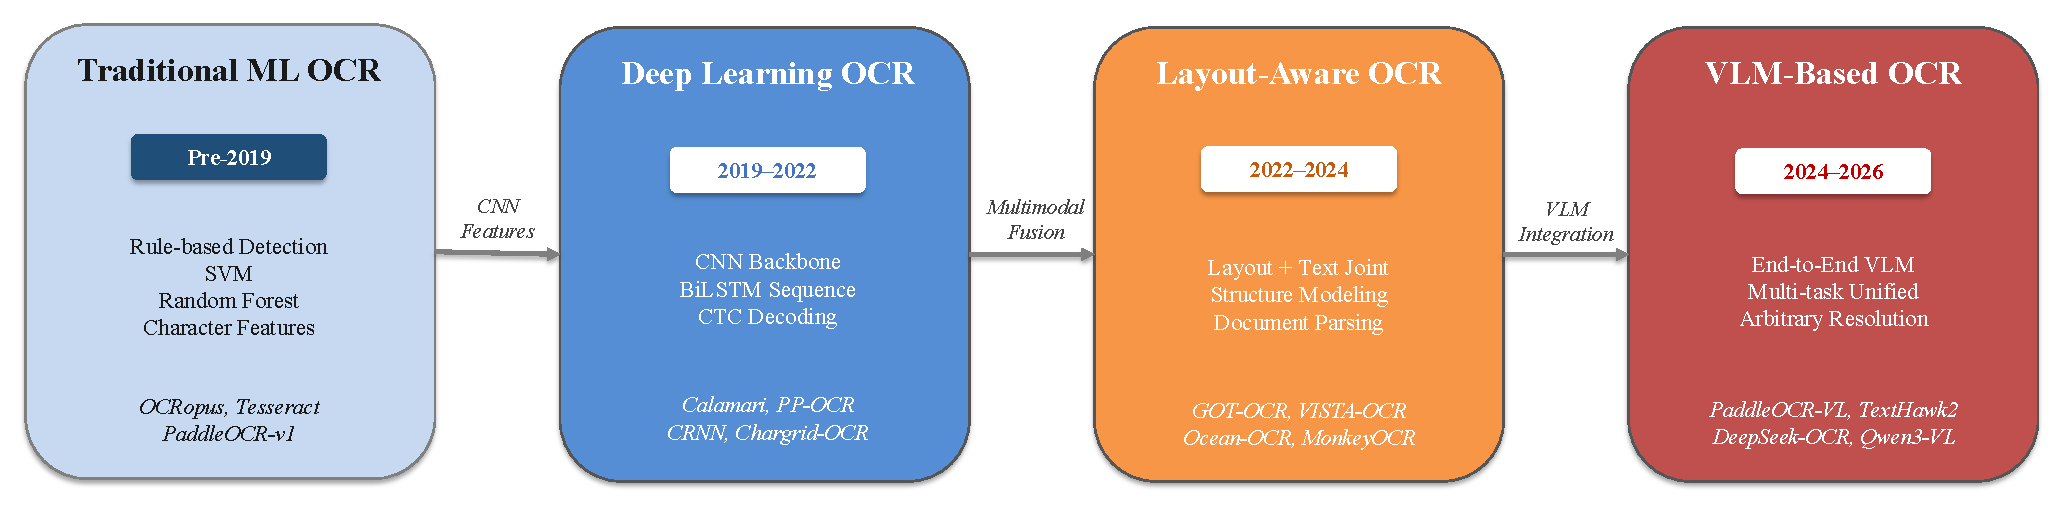
\includegraphics[
    width=0.95\textwidth,
    trim=0cm 0cm 0cm 0cm,
    clip
]{figs/fig02.pdf}
\caption{Four-stage evolution of optical character recognition technology (Pre-2019 to 2024--2026): from rule-based Traditional Machine Learning methods, through Deep Learning approaches with CNN--BiLSTM--CTC pipelines, to Layout-Aware OCR with joint structure modeling, and finally to Vision-Language Model-based OCR with end-to-end, multi-task unified frameworks.}
\label{fig:ocr_evolution}
\end{figure*}

\subsubsection{Layout Analysis and OCR Evaluation}

The evaluation landscape has evolved from task-driven to data-driven approaches. DocVQA \cite{mathew2020docvqa} constructed document visual question-answering tasks through large-scale question-document pairs. PubLayNet \cite{zhong2019publaynet} achieved layout annotation for over 360,000 pages by automatically aligning PDFs and XML files. DocLayNet \cite{pfitzmann2022doclaynet} provided over 80,000 pages of fine-grained human-annotated data from various fields.

For OCR specifically, OCRBench \cite{ocrbench2023} systematically revealed capability boundaries of large multimodal models across 29 sub-tasks. OmniDocBench \cite{omnidocbench2024} built a refined parsing benchmark covering nine document types. Recent datasets address linguistic diversity (SARD \cite{sard2025} for Arabic, 600k-ks-ocr \cite{ksocr2025} for Kashmiri), quality assessment (OCR-Quality \cite{ocrquality2025}), and domain specialization (PubMed-OCR \cite{pubmedocr2025} for scientific literature).
